\documentclass{article}
\usepackage[utf8]{inputenc}
\usepackage[margin=1.0in]{geometry}
\usepackage{graphicx}
\usepackage{wrapfig}
\usepackage{amsmath}
\usepackage[makeroom]{cancel}
\let\vec\mathbf
\usepackage{float}

\title{Optical Flow}
\author{George Tang, Neal Bayya}
\date{March 13, 2019}

\newcommand{\norm}[1]{\lvert #1 \rvert}
\newcommand*{\pd}[3][]{\ensuremath{\frac{\partial^{#1} #2}{\partial #3}}}

\begin{document}

\maketitle

\section{Introduction}
Optical flow allows us to track the motion of an object in a scene relative to an observer. Imagine the observer is standing at the center of a sphere and stares directly in front at a single point. Now imagine the sphere is spinning counterclockwise with respect to the observer. The observer views the motion of the sphere projected onto a 2D viewing plane. Over a short duration of time, each pixel is translated to a new location on the image due to the motion. In this case, we can calculate the optical flow and graphically draw it as the velocity vectors of the pixel (see figure below).

\begin{center}
    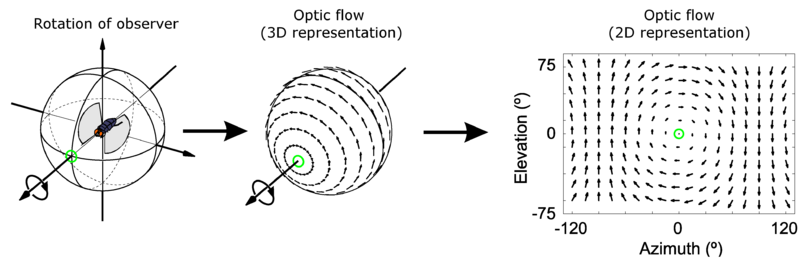
\includegraphics[width=0.8\textwidth]{optical1.png}
\end{center}
\noindent
There are numerous uses of optical flow, including navigation, reconstructing the depth of the object, and applications in computational photography. 

\section{Optical Flow}
Formally, given two images, one taken at $t_0$ and the other at $t_1$, we want to determine the motion of the pixels over time by looking at images $I_0$ and $I_1$. For instance, if we were given a video, we can compute a motion field by tracking the brightness patterns over successive frames. Before we discuss how to track the brightness, we must discuss the failure cases for optical flow. 
\\ \\
\begin{minipage}{.65\textwidth}
    \begin{itemize}
    \item Optical flow can only represent the \textit{apparent motion} of brightness patterns, meaning that it may not always yield the true motion.
    \item Deviation of apparent motion from true motion can be caused by variable lighting and other factors.
    \item Optical flow is limited to information contained in the frame.
    \item This results in optical flow suffering from the \text{Aperture Problem}, when motion along edges cannot be inferred. The figure on the right shows that although the motion is directed towards the down-right direction, optical flow will infer motion as to the right.
    \end{itemize}
\end{minipage}
\begin{minipage}{.35\textwidth}
\begin{center}
    \vspace{10pt}
    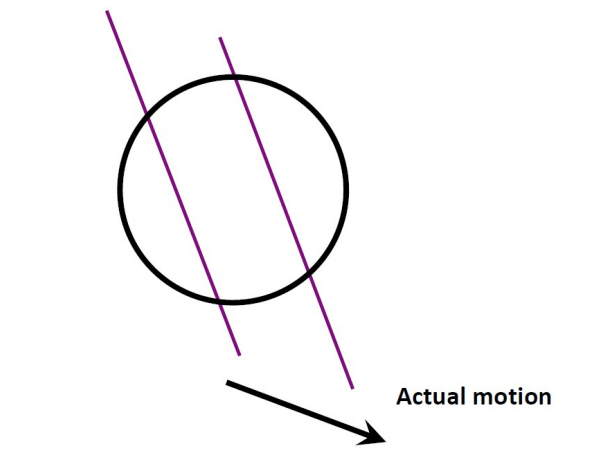
\includegraphics[width=1\textwidth]{apectureprob.png}
  \end{center}
\end{minipage}

\section{Brightness Constancy Constraint}
Because optical flow can only track apparent motion, we assume that the brightness of each pixel remains constant between frames. Mathematically, this is:

$$ I(x, y, t-1) = I(x+\Delta x, y+\Delta y, t)$$

\noindent
where $\Delta x$ and $\Delta y$ are the horizontal and vertical motions of the object and $t$ the timestamp. If we assume the motion is small, then we can setup a local linear approximation. To do so consider our brightness function:

$$ I(x(t), y(t), t)$$
\noindent
Taking the derivative (apply the chain rule for partial derivatives)

$$ \frac{dI(x(t), y(t), t)}{dt} = \frac{\partial I}{\partial x}\frac{dx}{dt} + \frac{\partial I}{\partial y}\frac{dy}{dt} + \frac{\partial I}{\partial t}$$

\noindent
So our approximation becomes

$$I(x+\Delta x, y+\Delta y, t) = I(x, y, t-1) + \frac{dI(x(t), y(t), t)}{dt} $$

$$I(x+\Delta x, y+\Delta y, t) = I(x, y, t-1) + \frac{\partial I}{\partial x}\frac{dx}{dt} + \frac{\partial I}{\partial y}\frac{dy}{dt} + \frac{\partial I}{\partial t}$$

\noindent
And because the brightness remains the same

$$ \frac{\partial I}{\partial x}\frac{dx}{dt} + \frac{\partial I}{\partial y}\frac{dy}{dt} + \frac{\partial I}{\partial t} = 0$$

$$ I_xu + I_yv + I_t  = 0$$
$$ I_xu + I_yv = -I_t$$

\noindent
where  $I_x$ is $\frac{\partial I}{\partial x}$, u = $\frac{dx}{dt}$, etc... Notice this yeilds two variables per pixel. If we assume a \textit{spatial coherence}, meaning that local pixels move in the same way (same $u$ and $v$), we can obtain a system of equations and solve for $u$ and $v$. How this is implemented is through the Lucas–Kanade Method.

\section{Lucas–Kanade Method}
In the Lucas–Kanade Method, instead of one equation from one pixel, we obtain many equations from a local patch of pixels that move in the same way (u and v are the same). For instance, we if use a 3 by 3 patch, then we will have 9 equations.

$$ I_x(x_0, y_0)u + I_y(x_0, y_0)v = -I_t(x_0, y_0)$$
$$ I_x(x_1, y_1)u + I_y(x_1, y_1)v = -I_t(x_1, y_1)$$
$$&\;\;\vdots \notag \\$$
$$ I_x(x_n, y_n)u + I_y(x_n, y_n)v = -I_t(x_n, y_n)$$
\\
\noindent
This system can be written in matrix form as $Am = b$
\begin{center}
\[ A =  \begin{bmatrix}
I_x(x_0, y_0) & I_y(x_0, y_0) \\
I_x(x_1, y_1) & I_y(x_1, y_1) \\
\;\;\vdots \notag  &  \;\;\vdots \notag \\
I_x(x_n, y_n)  & I_y(x_n, y_n)
\end{bmatrix} 
%
\hspace{10pt}
m = 
\begin{bmatrix}
u \\
v 
\end{bmatrix}
%
\hspace{10pt}
b = 
\begin{bmatrix}
-I_t(x_0, y_0) \\ 
-I_t(x_1, y_1) \\ 
\;\;\vdots \notag \\
-I_t(x_n, y_n)
\end{bmatrix}
\]
\end{center}
\noindent
The system has more equations than variables, which is known as an \textit{over-determined system}, meaning most likely it is inconsistent (has no solution). The Lucas–Kanade Method obtains a compromised solution using the least squares method ($A^T$ denotes the transpose of matrix $A$).

$$ Am = b $$
$$ A^TAm = A^Tb $$
$$ m = (A^TA)^{-1}A^Tb$$

\begin{center}
\[
\begin{bmatrix}
u \\ 
v 
\end{bmatrix}
% 
=
\begin{bmatrix}
\sum_i{I_x(x_i, y_i)^2} & \sum_i{I_x(x_i, y_i)I_y(x_i, y_i)} \\ 
\sum_i{I_x(x_i, y_i)I_y(x_i, y_i) & \sum_i{I_y(x_i, y_i)^2}
\end{bmatrix}
\begin{bmatrix}
-\sum_i{I_x(x_i, y_i)I_t(x_i, y_i)} \\
-\sum_i{I_y(x_i, y_i)I_t(x_i, y_i)}
\end{bmatrix}
\]
\end{center}
\section{Horn–Schunck Method}
The Horn-Schnuck Method is a second approach towards estimating optical flow in image sequences. Recall that we used an assumption that the flow is constant in a local neighborhood in the Lucas-Kanade method. Here, we assume \textit{smoothness} in the flow of brightness over the whole image. In the Horn-Schnuck method, we generate an energy function to model the distortion of flow and attempt to minimize it, thereby preferring solutions which show more smoothness. The energy function we are trying to minimize is formulated as:

$$E = \int \int \left[\left(I_xu + I_yv + I_t\right)^2  + \alpha^2 \left( \lvert \lvert \nabla u \rvert \rvert^2  + \lvert \lvert \nabla v \rvert \rvert^2\right) \right]dxdy$$
\noindent
where $I_x, I_y, I_t$ are the image intensity derivatives with respect to  x, y, and time, respectively. The vector $\mathbf{V} = \left[ u(x,y), v(x,y) \right]$ is the optical flow vector and represents the velocity vectors of the pixels. Recall that the Brightness Constancy Model for Optical flow states that $ I_xu + I_yv + I_t  = 0$. In minimizing our energy function, we are searching for the velocity components $u$ and $v$ that get the first integrand expression as close to 0 as possible. $\alpha$ is a regularization parameter which controls the smoothness of the optical flow. Larger values of $\alpha$ will lead to greater smoothness because we are forcing the $\left( \lvert \lvert \nabla u \rvert \rvert^2  + \lvert \lvert \nabla v \rvert \rvert^2\right)$ expression to decrease to minimize energy, which has the effect of reducing the velocities of the pixels.\\
\noindent
To minimize the energy function, $E$, we can focus on minimizing the integrand, which we will call $L$.

$$L = \left(I_xu + I_yv + I_t\right)^2  + \alpha^2 \left( \lvert \lvert \nabla u \rvert \rvert^2  + \lvert \lvert \nabla v \rvert \rvert^2\right)$$
\noindent
We can minimize $L$ by differentiating the function with respect to our two unknowns ($u$ and $v$) and setting them equal to 0 because we know that local extrema occur where the partial derivatives 0. Differentiating $L$ with respect to $u$ and $v$ yield the following two equations: 

$$I_x \left( I_xu + I_yv + I_t \right) - \alpha^2\Delta u = 0 $$
$$I_y \left( I_xu + I_yv + I_t \right) - \alpha^2\Delta v = 0 $$
\noindent
where $\Delta = \pd[2]{}{x^2} + \pd[2]{}{y^2}$ is called the Lagrangian operator, which in practice is computed as 
$$\Delta u(x,y) = \bar{u}(x,y) - u(x,y)$$
\noindent
where $\bar{u}(x,y)$ is a weighted average of $u$ in a neighborhood around $(x,y)$. Substituting this expression for the Lagrangian operator back into the two equations above yields
$$ \left( {I_x}^2 + \alpha^2 \right) u + I_xI_yv = \alpha^2\bar{u} - I_xI_t $$
$$ I_xI_yu + \left( {I_y}^2 + \alpha^2 \right)v = \alpha^2 \bar{v} -I_yI_t $$
\noindent
which gives us linear models to solve for $u$ and $v$ for each pixel.



\end{document}


